%-----------------------------------------------------------------------------------------------%
%
% Maret 2019
% Template Latex untuk Tugas Akhir Program Studi Sistem informasi ini
% dikembangkan oleh Inggih Permana (inggihjava@gmail.com)
%
% Template ini dikembangkan dari template yang dibuat oleh Andreas Febrian (Fasilkom UI 2003).
%
% Orang yang cerdas adalah orang yang paling banyak mengingat kematian.
%
%-----------------------------------------------------------------------------------------------%

%-----------------------------------------------------------------------------%
%\prefikLampiran{A}

\renewcommand{\thepage}{D - \arabic{page}}
\chapter{\textit{SOURCE CODE} / Use Case Diagram / Activity Diagram / Database / Interface}
%-----------------------------------------------------------------------------%
\begin{figure}[h]
	\centering
	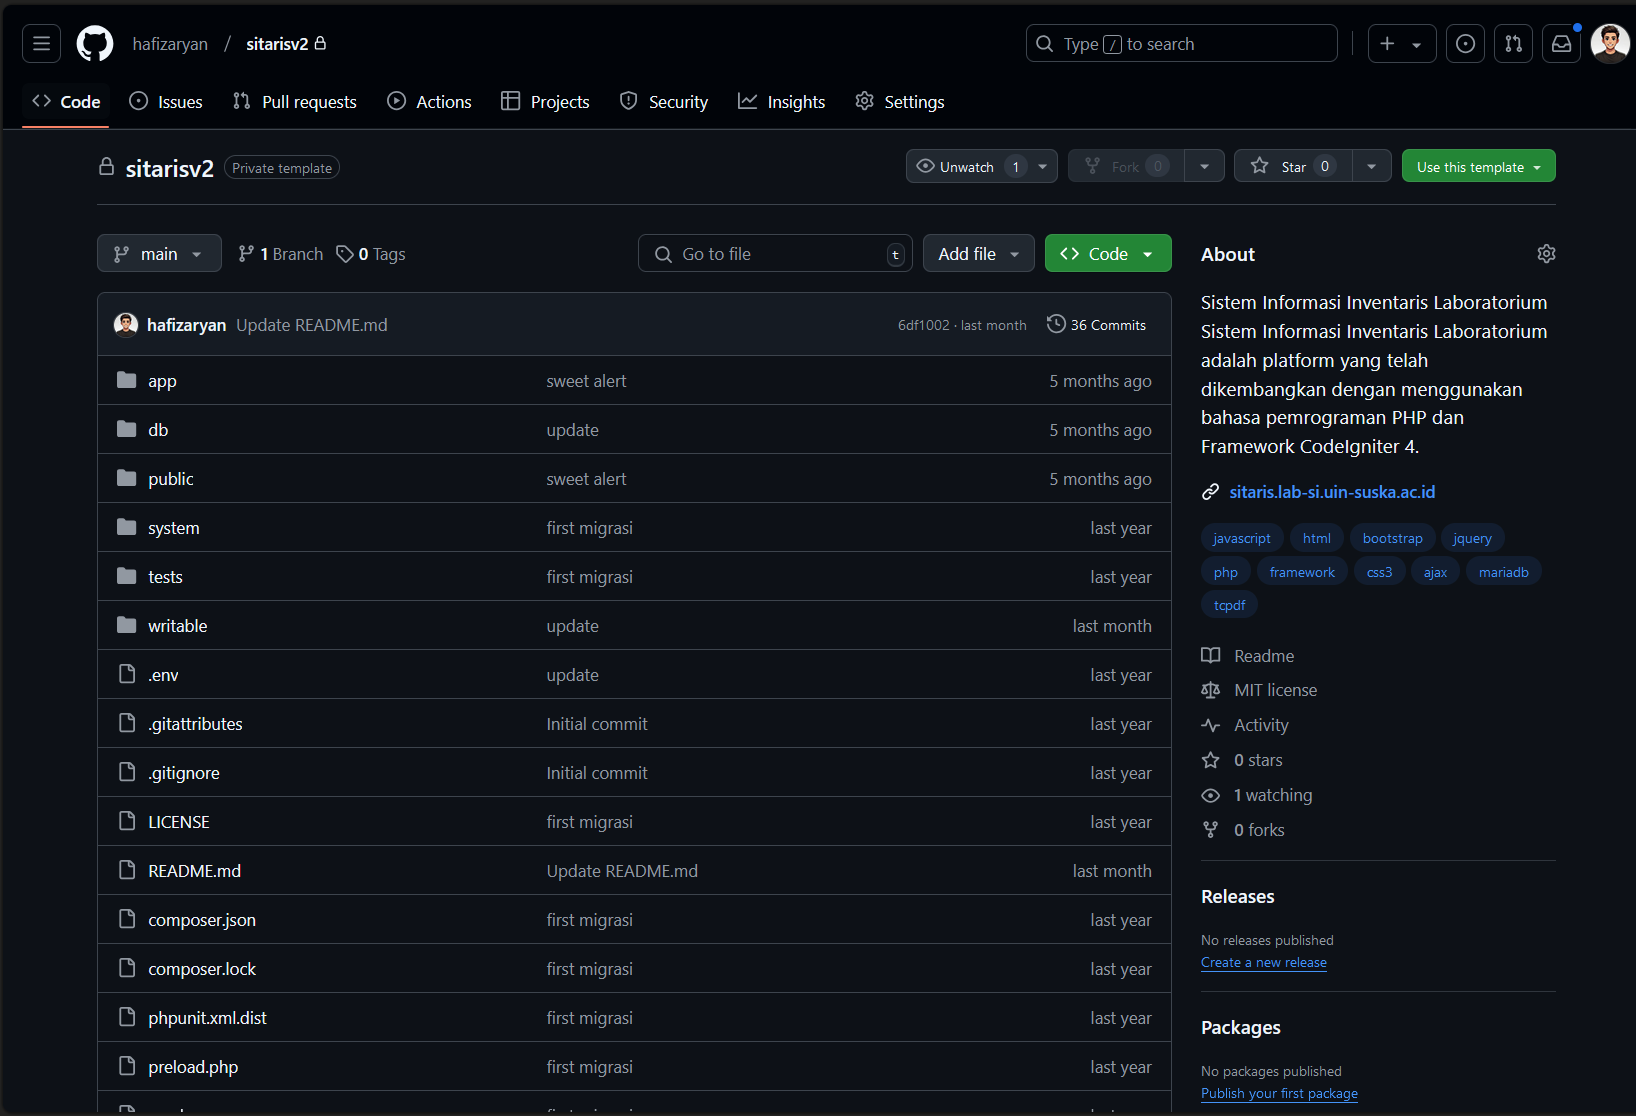
\includegraphics[width=0.82\linewidth]{konten/gambar/source-code.png}
	\caption{\textit{Source Code}}
	\label{fig:source-code}
\end{figure}

\begin{figure}
	\centering
	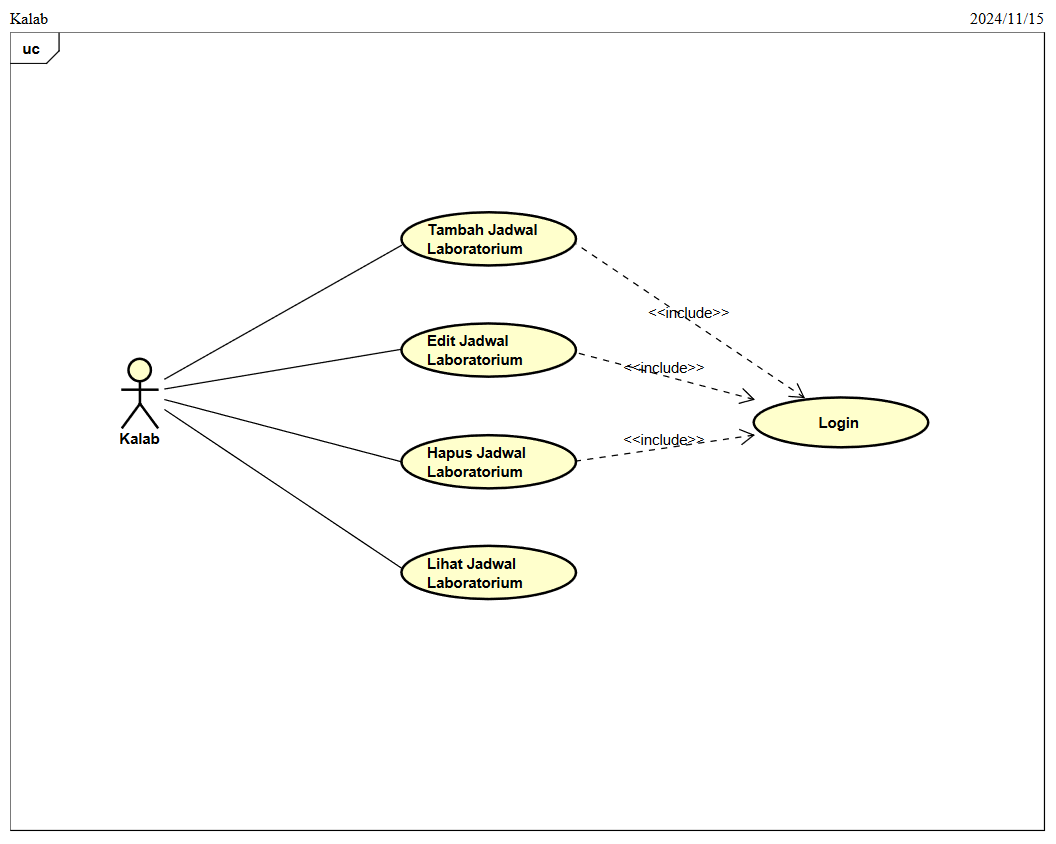
\includegraphics[width=0.82\textwidth]{konten/gambar/usecase-diagram/kalab.png}
	\caption{\textit{Usecase Diagram} Kalab}
	\label{usecase-diagram-kalab}
\end{figure}

\begin{figure}
	\centering
	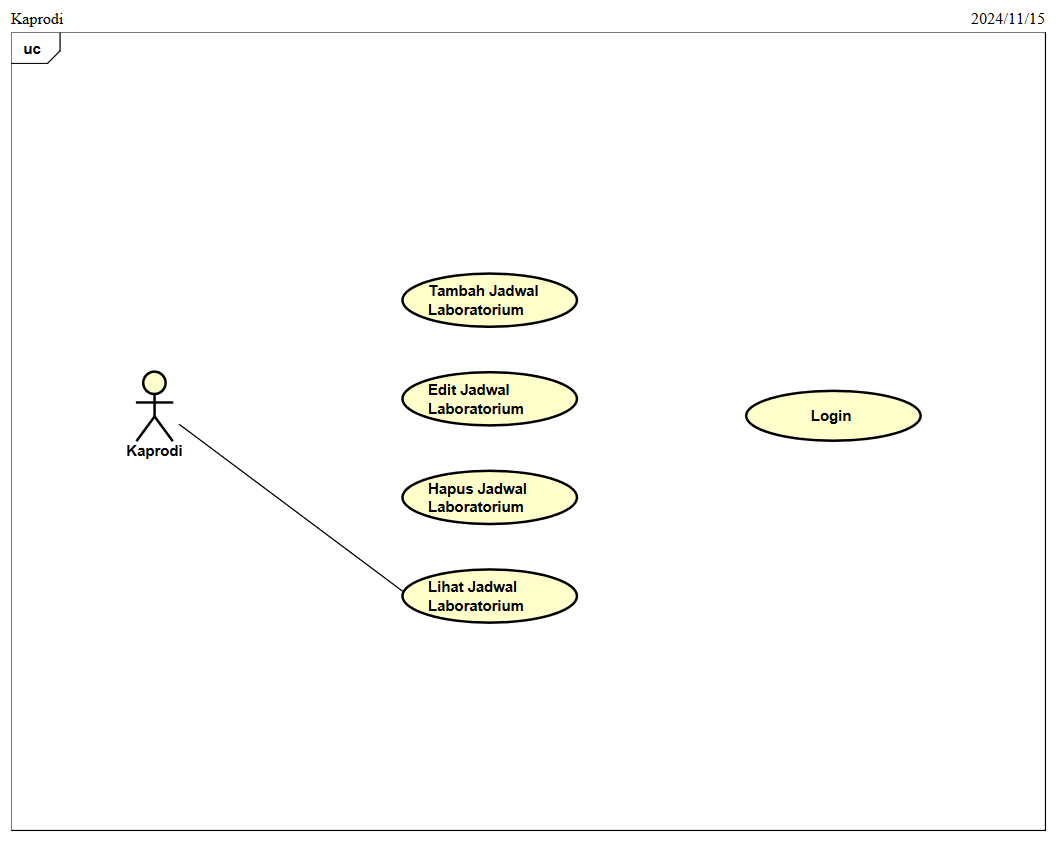
\includegraphics[width=0.82\textwidth]{konten/gambar/usecase-diagram/kaprodi.png}
	\caption{\textit{Usecase Diagram} Kaprodi}
	\label{usecase-diagram-kaprodi}
\end{figure}

\begin{figure}
	\centering
	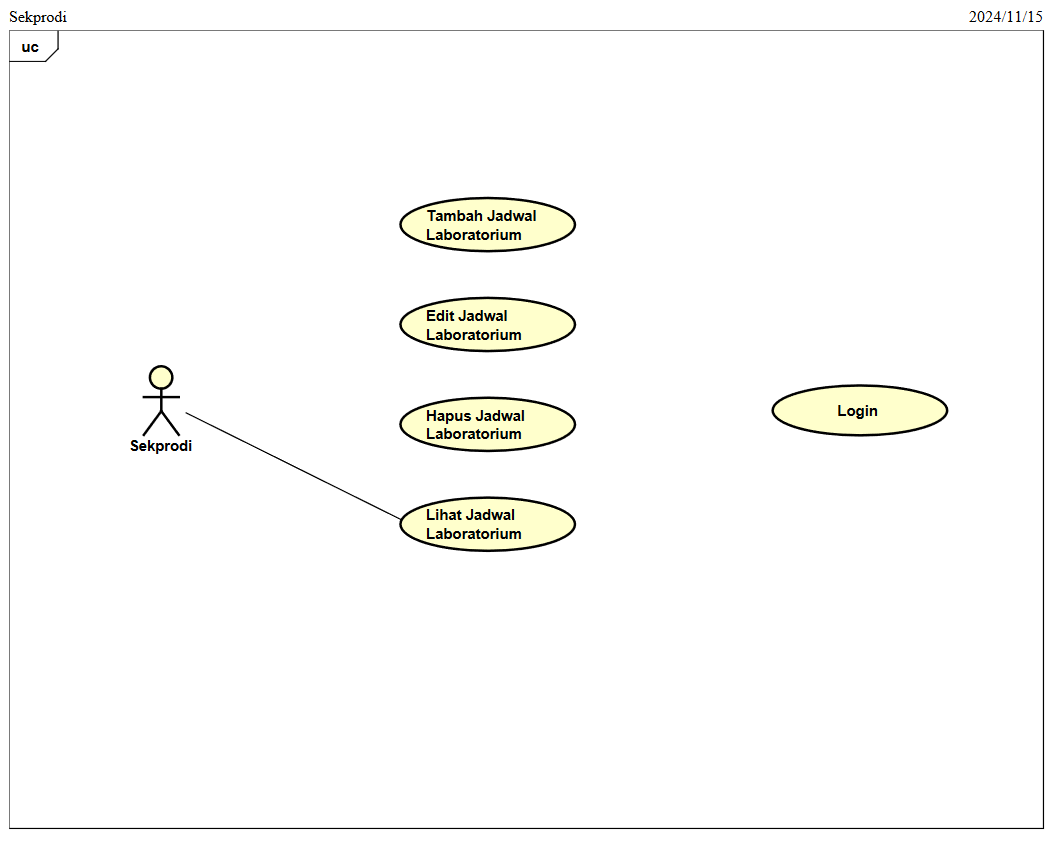
\includegraphics[width=0.82\textwidth]{konten/gambar/usecase-diagram/sekprodi.png}
	\caption{\textit{Usecase Diagram} Sekprodi}
	\label{usecase-diagram-sekprodi}
\end{figure}

\begin{figure}
	\centering
	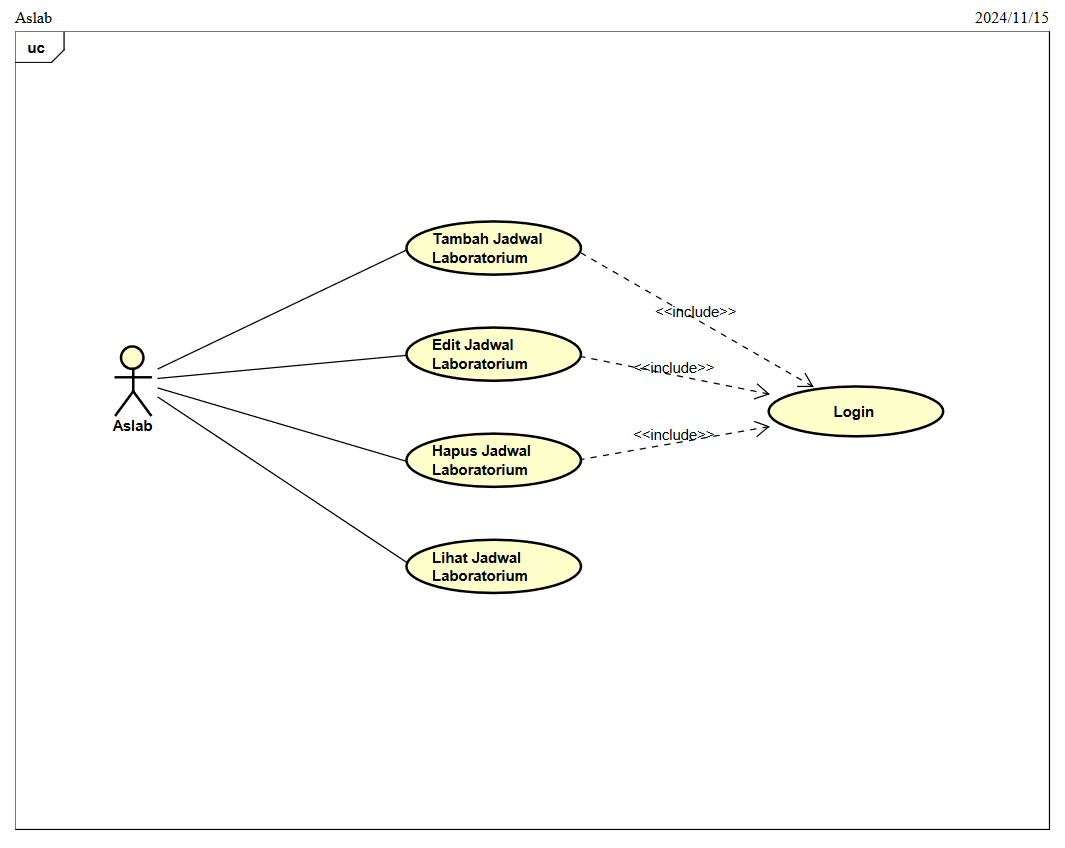
\includegraphics[width=0.82\textwidth]{konten/gambar/usecase-diagram/aslab.png}
	\caption{\textit{Usecase Diagram} Aslab}
	\label{usecase-diagram-aslab}
\end{figure}

\begin{figure}
	\centering
	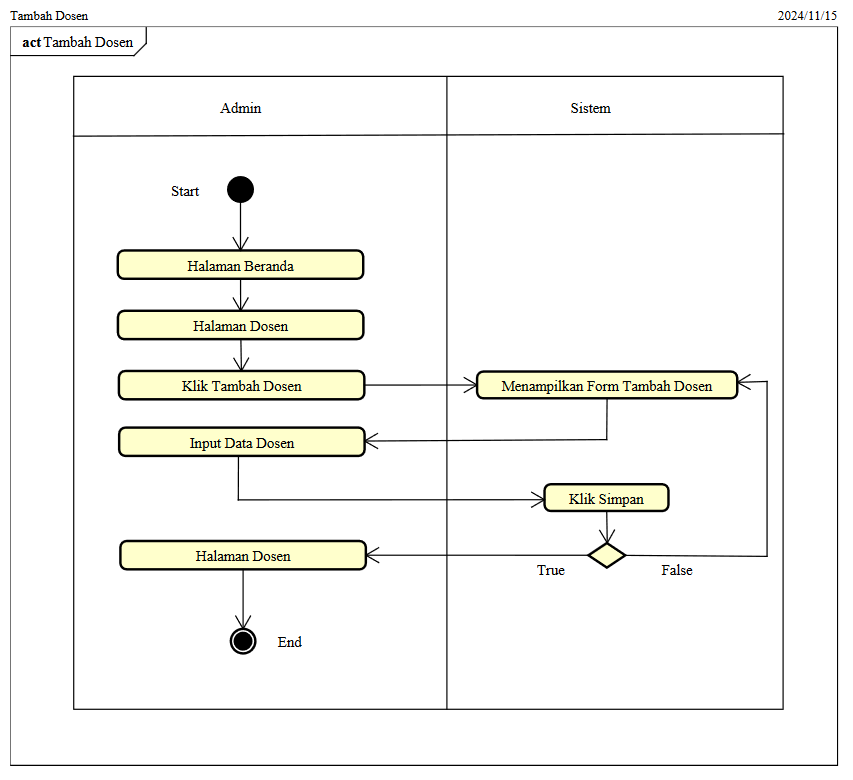
\includegraphics[width=0.82\textwidth]{konten/gambar/activity-diagram/tambah-dosen.png}
	\caption{\textit{Activity Diagram} Tambah Dosen}
	\label{activity-diagram-tambah-dosen}
\end{figure}

\begin{figure}
	\centering
	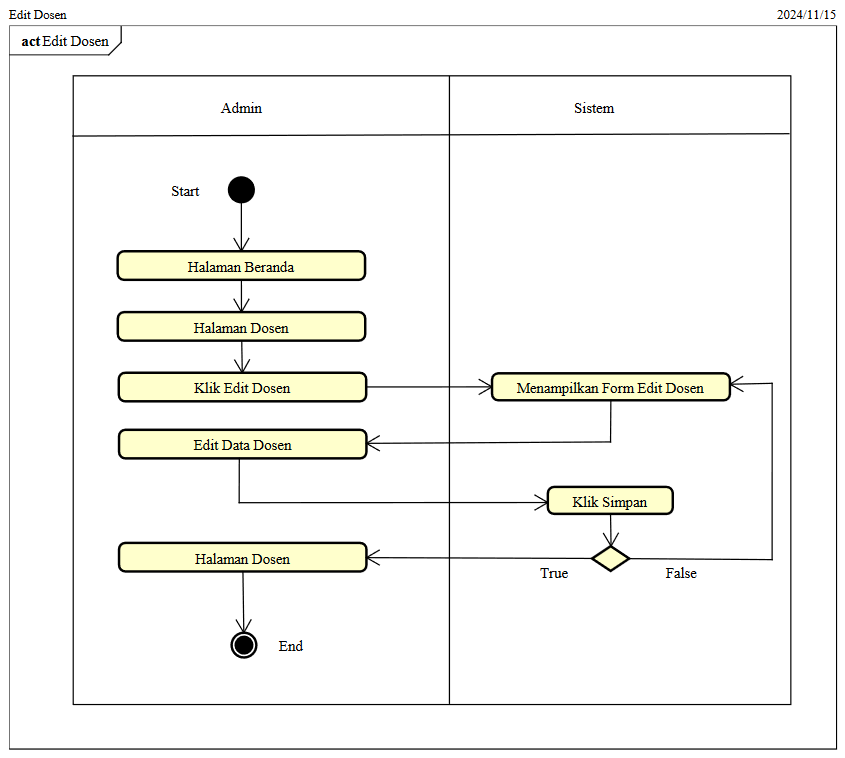
\includegraphics[width=0.82\textwidth]{konten/gambar/activity-diagram/edit-dosen.png}
	\caption{\textit{Activity Diagram} Edit Dosen}
	\label{activity-diagram-edit-dosen}
\end{figure}

\begin{figure}
	\centering
	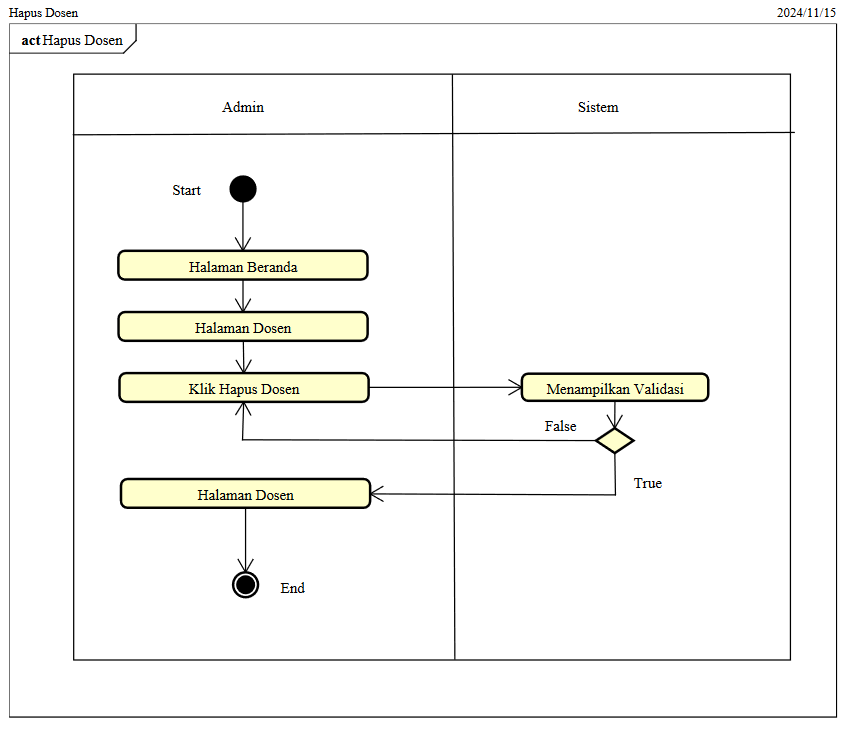
\includegraphics[width=0.82\textwidth]{konten/gambar/activity-diagram/hapus-dosen.png}
	\caption{\textit{Activity Diagram} Hapus Dosen}
	\label{activity-diagram-hapus-dosen}
\end{figure}

\begin{figure}
	\centering
	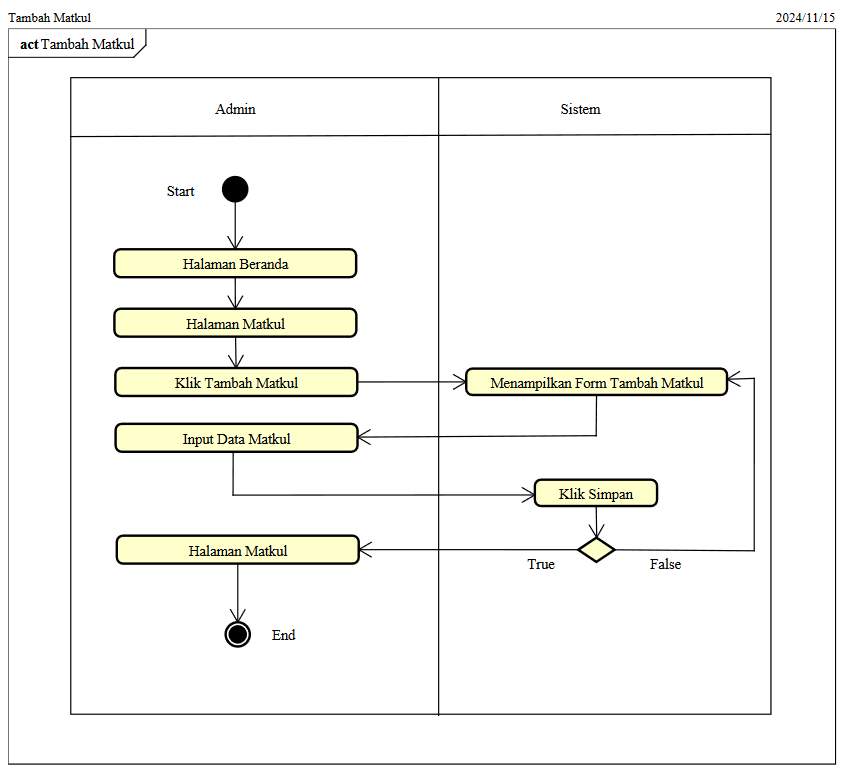
\includegraphics[width=0.82\textwidth]{konten/gambar/activity-diagram/tambah-matkul.png}
	\caption{\textit{Activity Diagram} Tambah Mata Kuliah}
	\label{activity-diagram-tambah-matkul}
\end{figure}

\begin{figure}
	\centering
	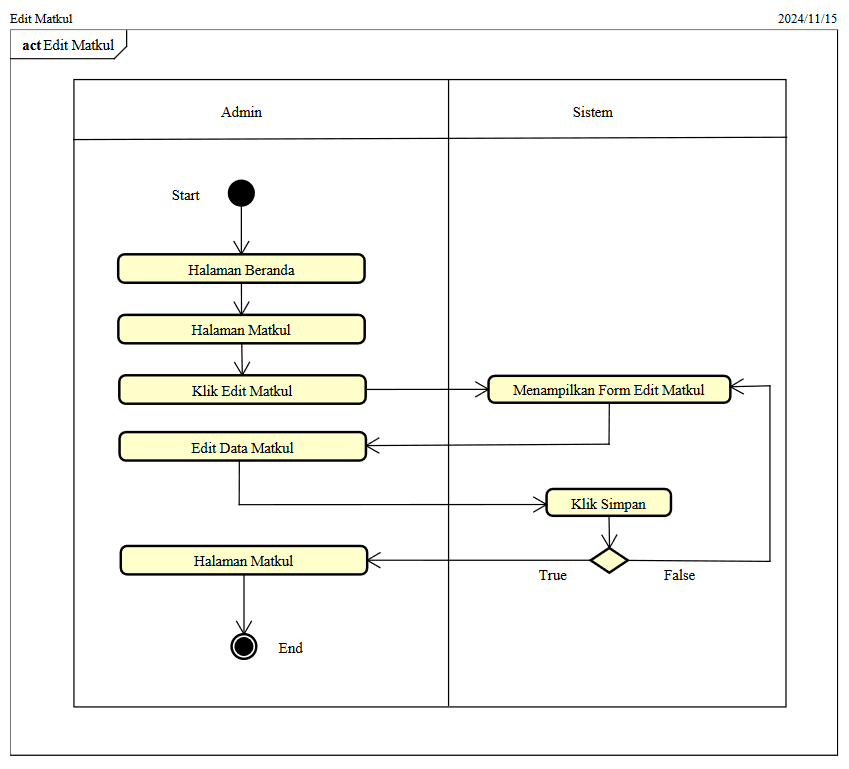
\includegraphics[width=0.82\textwidth]{konten/gambar/activity-diagram/edit-matkul.png}
	\caption{\textit{Activity Diagram} Edit Mata Kuliah}
	\label{activity-diagram-edit-matkul}
\end{figure}

\begin{figure}
	\centering
	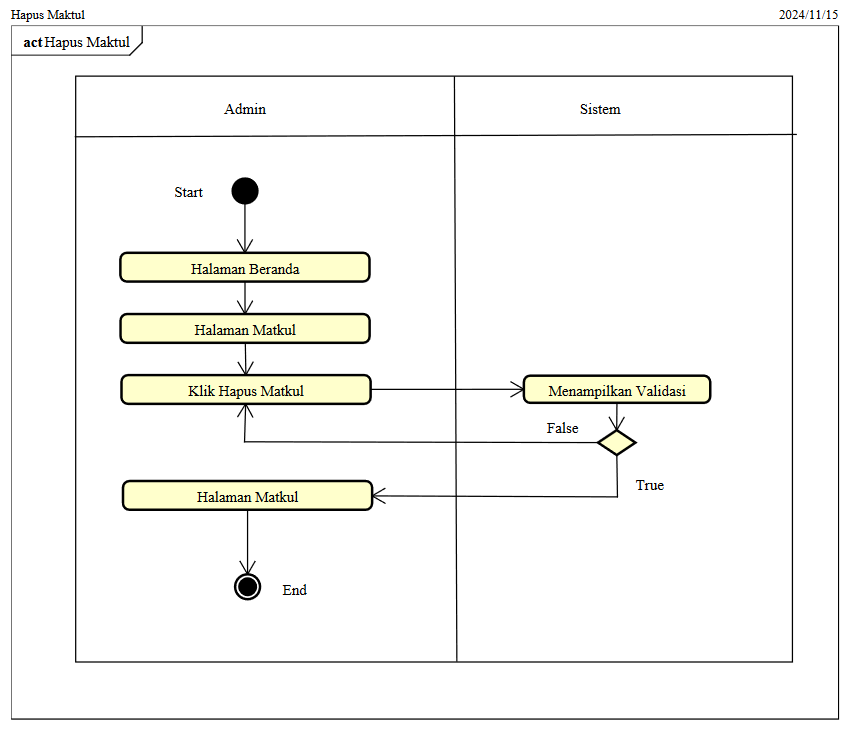
\includegraphics[width=0.82\textwidth]{konten/gambar/activity-diagram/hapus-matkul.png}
	\caption{\textit{Activity Diagram} Hapus Mata Kuliah}
	\label{activity-diagram-hapus-matkul}
\end{figure}

\begin{figure}
	\centering
	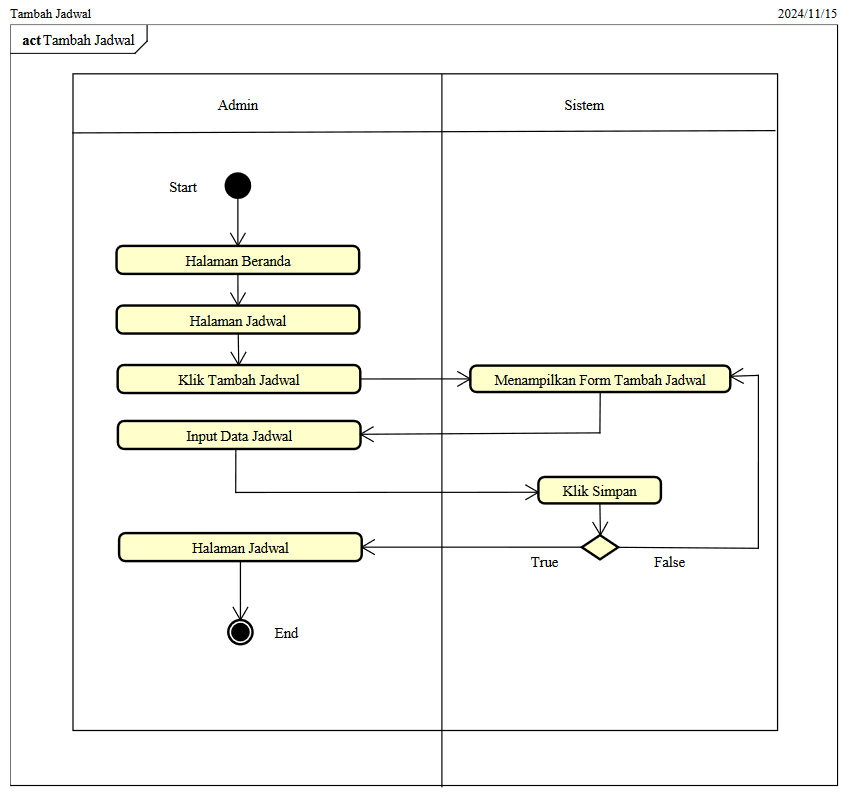
\includegraphics[width=0.82\textwidth]{konten/gambar/activity-diagram/tambah-jadwal.png}
	\caption{\textit{Activity Diagram} Tambah Jadwal}
	\label{activity-diagram-tambah-jadwal}
\end{figure}

\begin{figure}
	\centering
	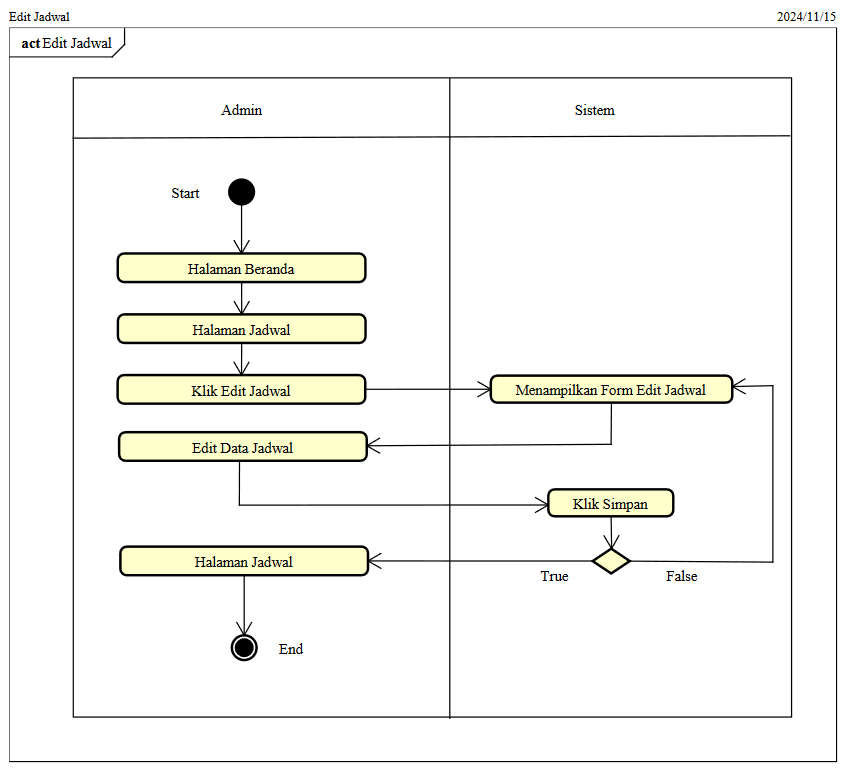
\includegraphics[width=0.82\textwidth]{konten/gambar/activity-diagram/edit-jadwal.png}
	\caption{\textit{Activity Diagram} Edit Jadwal}
	\label{activity-diagram-edit-jadwal}
\end{figure}

\begin{figure}
	\centering
	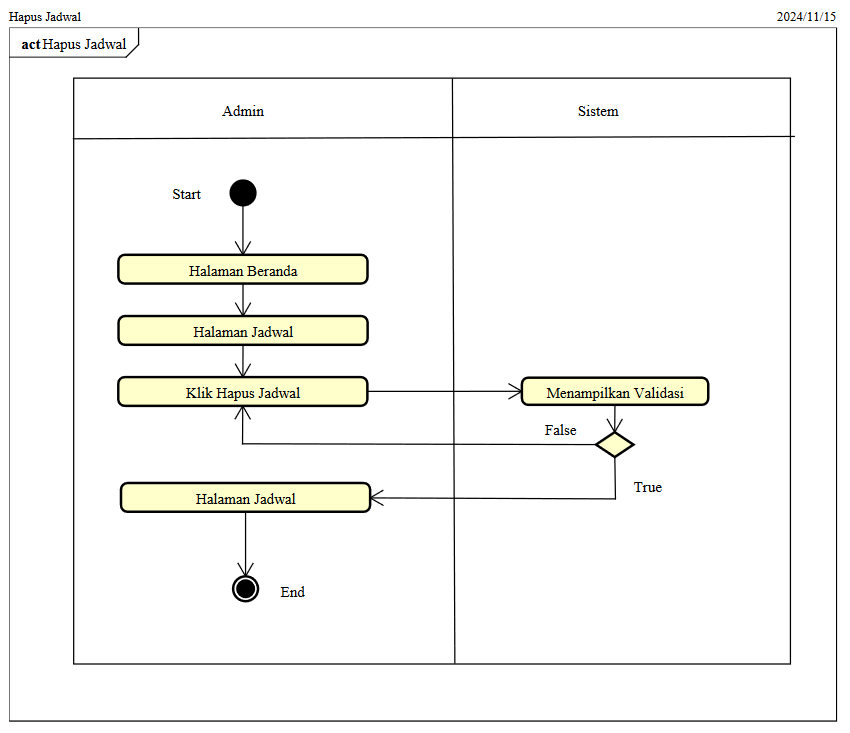
\includegraphics[width=0.82\textwidth]{konten/gambar/activity-diagram/hapus-jadwal.png}
	\caption{\textit{Activity Diagram} Hapus Jadwal}
	\label{activity-diagram-hapus-jadwal}
\end{figure}

\begin{figure}
	\centering
	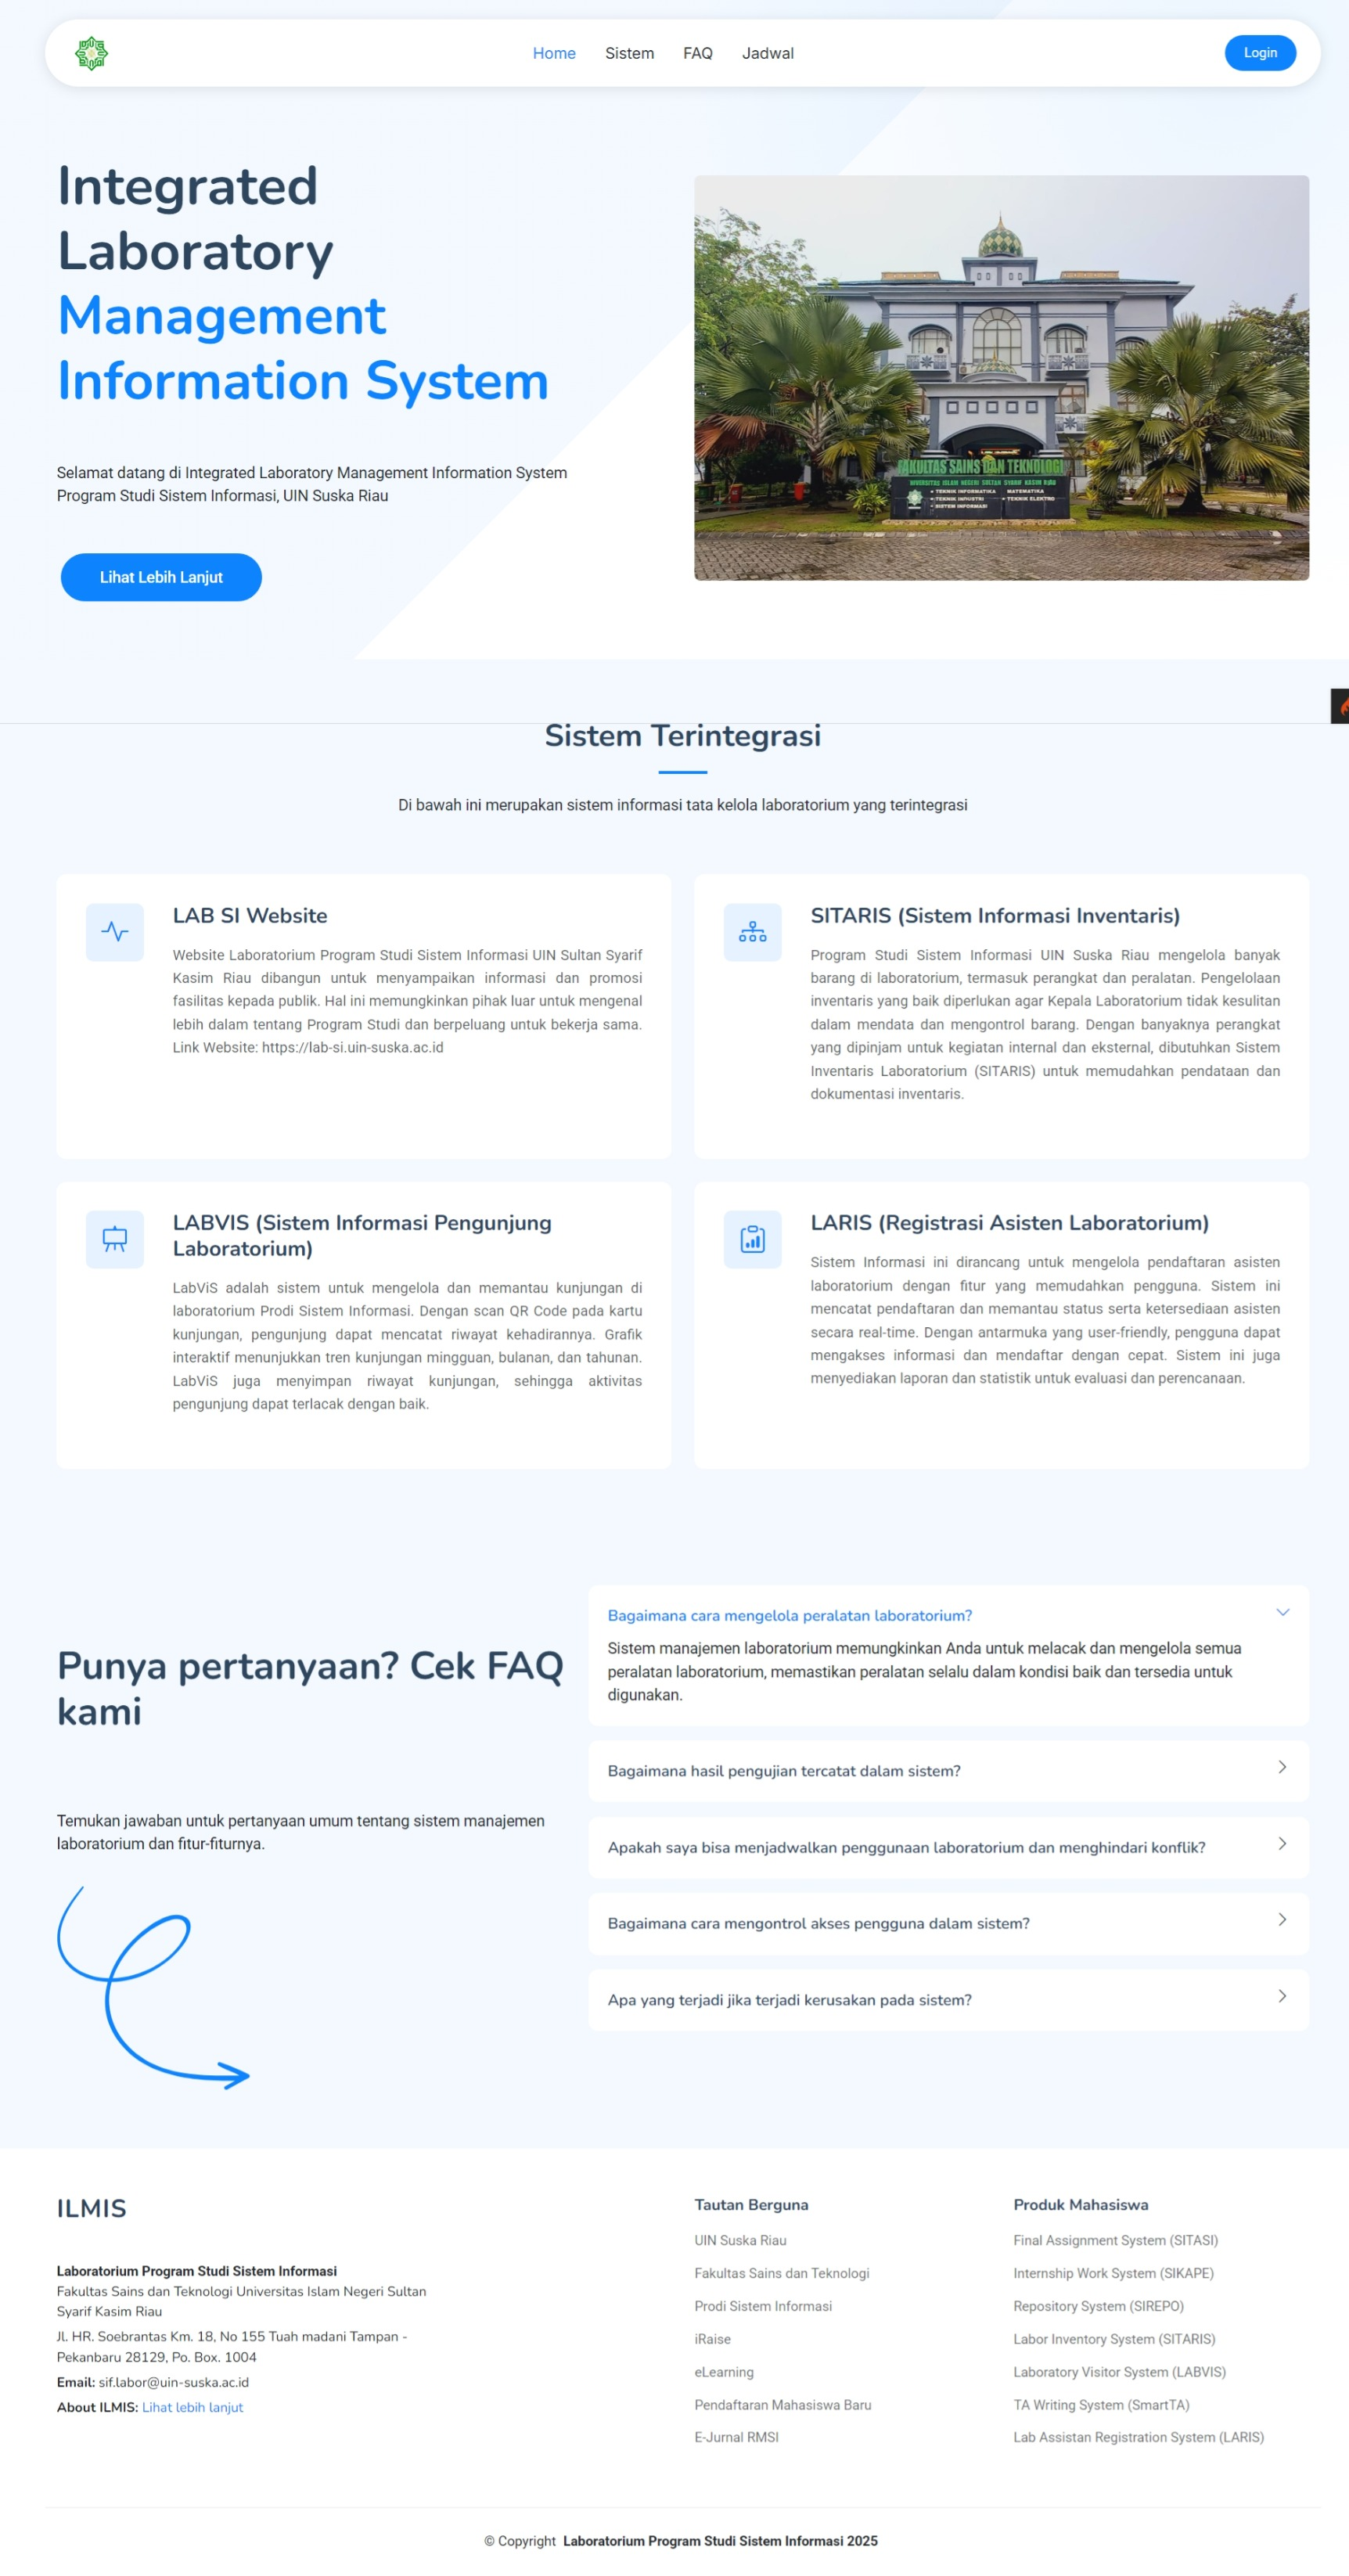
\includegraphics[width=0.82\textwidth]{konten/gambar/hasil/landing-page.jpeg}
	\caption{Tampilan \textit{Landing Page} Sistem Manajemen Laboratorium}
	\label{fig:landing-page}
\end{figure}

\begin{figure}
	\centering
	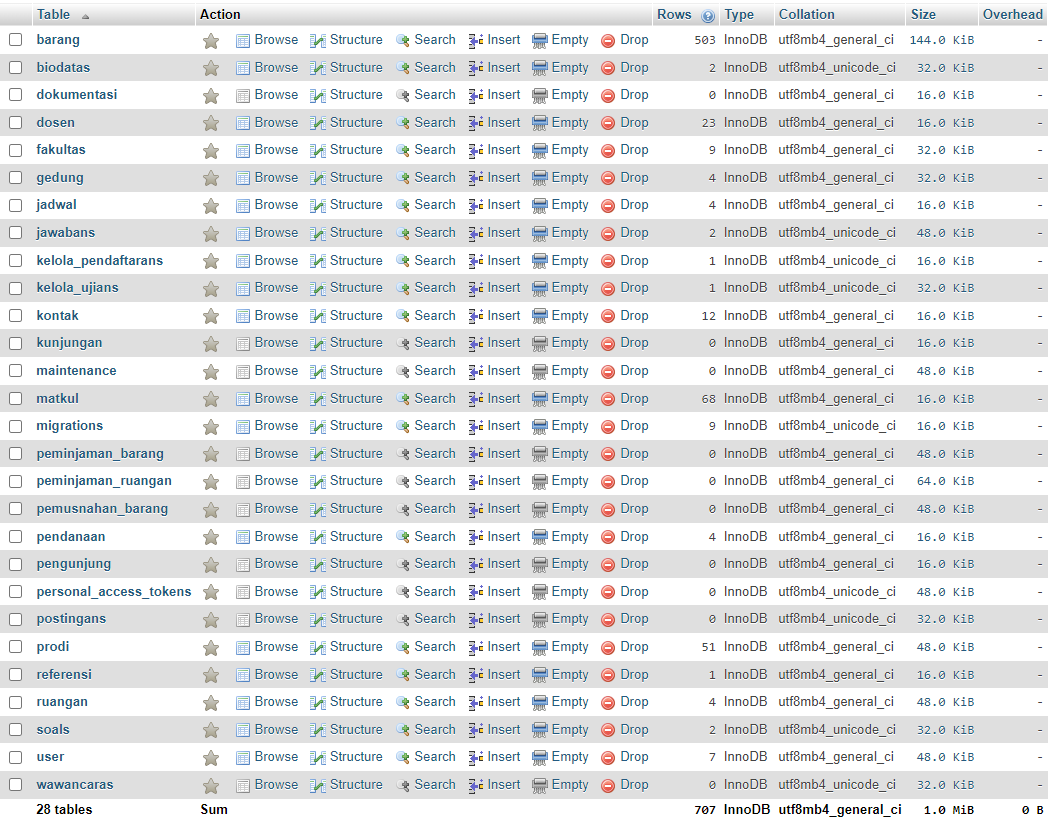
\includegraphics[width=0.82\textwidth]{konten/gambar/implementasi/database.png}
	\caption{\textit{Database}}
	\label{database-manlab}
\end{figure}

\begin{figure}
	\centering
	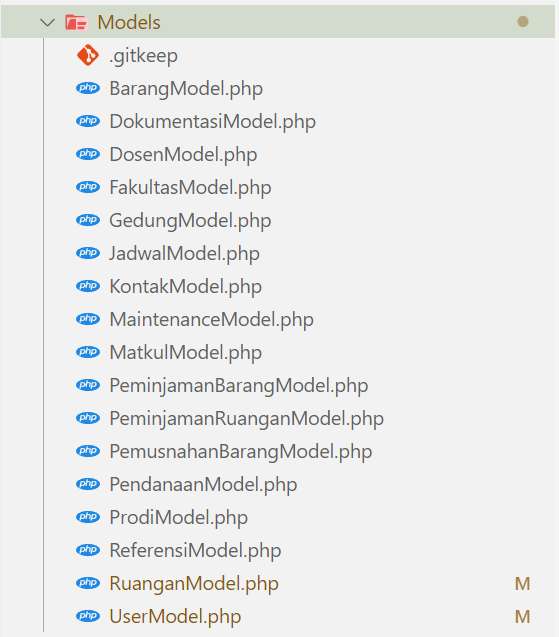
\includegraphics[width=0.82\linewidth]{konten//gambar/implementasi-folder/folder-model.png}
	\caption{Implementasi Model}
	\label{fig:implementasi-model}
\end{figure}

\begin{figure}
	\centering
	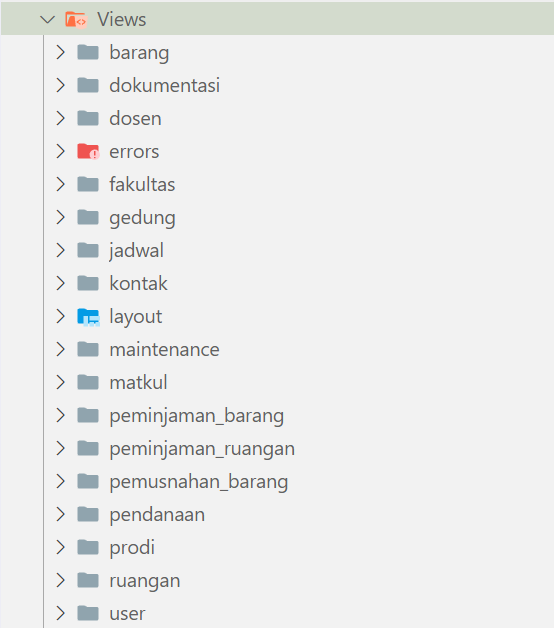
\includegraphics[width=0.82\linewidth]{konten//gambar/implementasi-folder/folder-view.png}
	\caption{Implementasi View}
	\label{fig:implementasi-view}
\end{figure}

\begin{figure}
	\centering
	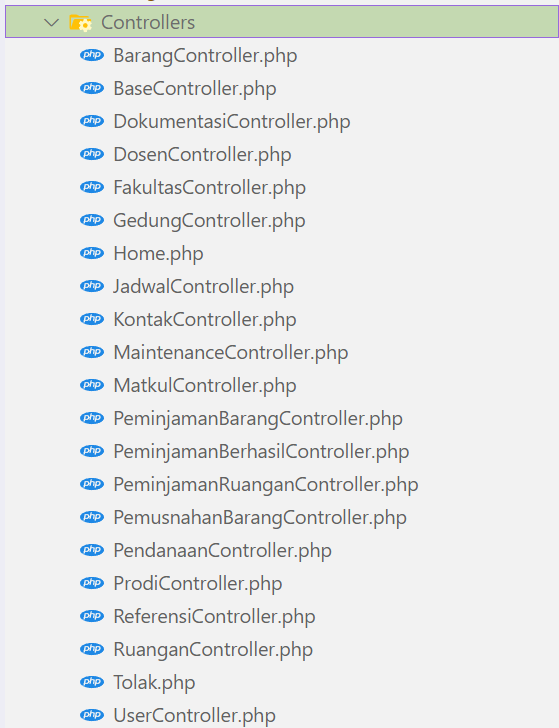
\includegraphics[width=0.82\linewidth]{konten//gambar/implementasi-folder/folder-controller.png}
	\caption{Implementasi Controller}
	\label{fig:implementasi-controller}
\end{figure}
